\subsection{Analysis}
\label{sec:dcqcn_stability}

\begin{figure*}[t]
\subfigure[Default parameters ($R_{AI}=40Mbps$, $K_{max}=200KB$).]
{
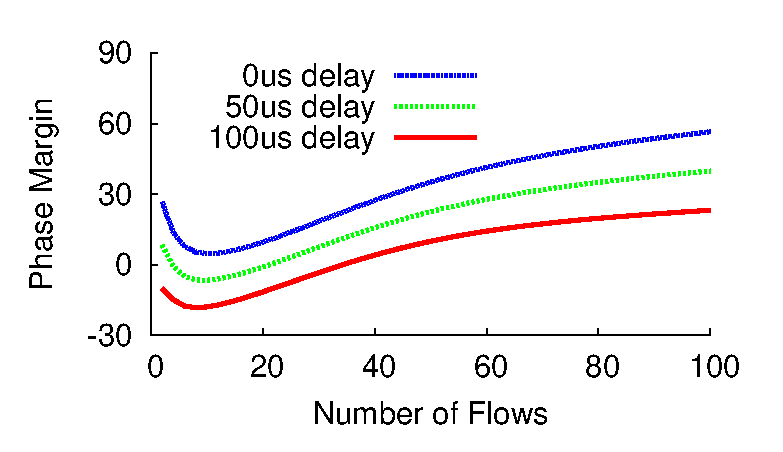
\includegraphics[width=0.33\textwidth]{figures/dcqcn_stability.eps}
\label{fig:dcqcn_stability_default}
}
\subfigure[$R_{AI}=10Mbps$.]
{
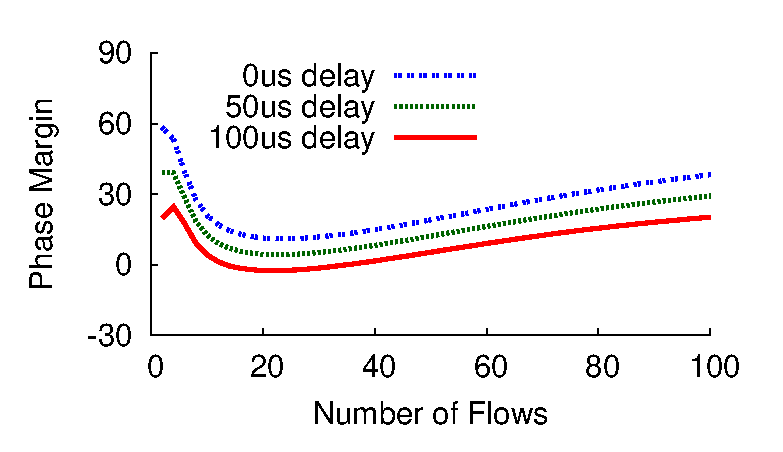
\includegraphics[width=0.33\textwidth]{figures/dcqcn_stability_rai.eps}
\label{fig:dcqcn_stability_rai}
}
\subfigure[$R_{AI}=10Mbps$ and $K_{max}=1000KB$.]
{
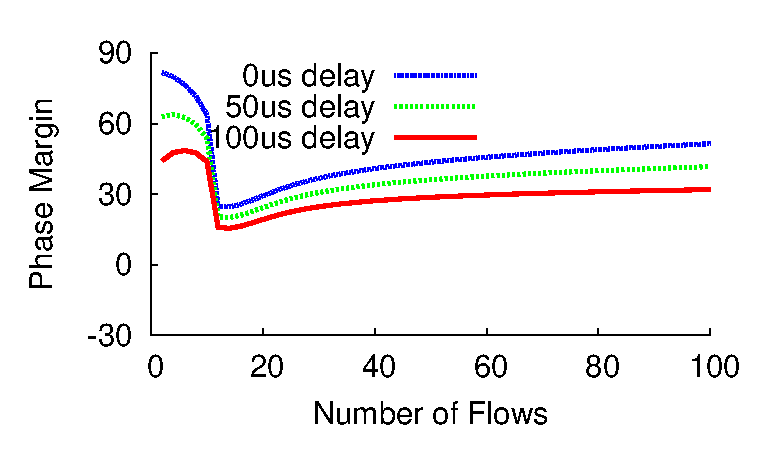
\includegraphics[width=0.33\textwidth]{figures/dcqcn_stability_rai_kmax.eps}
\label{fig:dcqcn_stability_rai_kmax}
}
\caption{DCQCN stability}
\label{fig:dcqcn_stability}
\end{figure*}

A primary application of fluid models is to perform control theoretic analysis.
The first step in performing the analysis is to obtain the fixed point of the
system, so we can linearize the model about the fixed point and perform
classical frequency domain analysis. 

We now prove that DCQCN has a unique fixed point at which all flows converge to
the same rate. Then, we analyze DCQCN's stability around the fixed point,
focusing on whether DCQCN remains stable under different conditions. We conclude
with a parameter setting guidelines.

\para{Fixed point:} By setting the left-hand side of Equation~\ref{eq:q} to 0,
it is easy to see that any fixed points of the DCQCN (if they exist) must
satisfy:
\begin{equation}
\small
\sum\limits_{i = 1}^N {R_C^{(i)}(t)} = C
\label{eq:fixedrc}
\end{equation}
At any of the fixed points, we assume the value of $p$ is $p^*$, which is shared
by all flows. The queue length and per-flow $\alpha^{(i)}$ at the fixed points
are determined by Equation~\ref{eq:mark} and \ref{eq:alpha}:
\begin{equation}
\small
{q^*} = \frac{{{p^*}}}{{{p_{max}}}}\left( {{K_{max}} - {K_{min}}} \right) + {K_{min}}
\end{equation}
\begin{equation}
\small
\alpha^{(i)*}  = 1 - {(1 - p^*)^{{\tau '}R_C^{(i)*}}}
\end{equation}
Next, we show that $p^*$ exists and is uniquely determined by $R_C^{(i)*}$ in
the DCQCN model.  From Equation~\ref{eq:rt} and \ref{eq:rc}, at the fixed point,
we get the two forms of $R_T^{(i)*}$, respectively:
\begin{equation}
\small
{R_T^{(i)*}} = R_C^{(i)*} + \frac{{a\alpha^{(i)*} }}{{(b + d)\tau }}
\end{equation}
\begin{equation}
\small
{R_T^{(i)*}} = R_C^{(i)*}\left( {1 + \frac{{(c + e)\tau {R_{AI}}}}{a}} \right)
\end{equation}
Where we denote $a, b, c, d, e$ as follows:
\begin{equation}
\small
\begin{array}{l}
a = 1 - {(1 - p^*)^{\tau {R_C^{(i)*}}}},b = \frac{{p^*}}{{{{(1 - p^*)}^{ - B}} - 1}},c = \frac{{{{(1 - p^*)}^{FB}}p^*}}{{{{(1 - p^*)}^{ - B}} - 1}},\\
d = \frac{{p^*}}{{{{(1 - p^*)}^{ - T{R_C^{(i)*}}}} - 1}},e = \frac{{{{(1 - p^*)}^{FT{R_C^{(i)*}}}}p^*}}{{{{(1 - p^*)}^{ - T{R_C^{(i)*}}}} - 1}}
\end{array}
\end{equation}
Combining the two forms of $R_T^{(i)*}$, we see that the value of $p^*$ is determined by:
\begin{equation}
\small
\frac{{{a^2}\alpha^{(i)*} }}{{(b + d)(c + e)}} = {\tau ^2}{R_{AI}}R_C^{(i)*}
\label{eq:p_fixed}
\end{equation}
It is easy to see that the left-hand side of the above equation is monotonic when
$p \in [0,1]$: when $p = 0$, the left-hand side of Equation~\ref{eq:p_fixed} is
smaller than the right-hand side, while is vice versa when $p = 1$. Thus DCQCN
has a unique fixed point, determined by a unique $p^*$. 

The value of $p^*$ can be estimated using numerical approaches, and we find that
it is very close to 0. Therefore, we can obtain the taylor series around $p=0$
of the left-hand side:
\begin{equation}
\small
\frac{{{a^2}\alpha }}{{(b + d)(c + e)}} = \frac{{(R_C^{(i)*})^3{\tau ^2}\tau '}}{{{{\left( {\frac{1}{B} + \frac{1}{{TR_C^{(i)*}}}} \right)}^2}}}{p^3} + O\left( {{p^4}} \right)
\end{equation}
Omitting the $O(p^4)$ term, combining Equation~\ref{eq:p_fixed}, we have the fixed point of $p$:
\begin{equation}
\small
{p^*} = \sqrt[3]{{\frac{{{R_{AI}}}}{{{\tau '}(R_C^{(i)*})^2}}{{\left( {\frac{1}{B} + \frac{1}{TR_C^{(i)*}}} \right)}^2}}}
\label{eq:fixedp}
\end{equation}
From the equation above, we see that $p^*$ and $R_C^{(i)*}$ uniquely determine each other. 
Since $p^*$ is shared by any flow $i$, $i = 1, 2, ..., N$, we have:
\begin{equation}
\small
R_C^{(1)*} = R_C^{(2)*} = ... = R_C^{(N)*}
\end{equation}
Combining equation~\ref{eq:fixedrc}, we know that there is only one unique fixed
point, at which $R_C^{(i)*} = \frac{C}{N}$, $i = 1, 2, ..., N$ and $p^*$ is
given by equation~\ref{eq:fixedp}.


\para{Stability analysis.} 
We linearize the system by denoting $\delta {R_C}(t) = {R_C}(t) - R_C^*$,
$\delta {R_C}(t) = {R_C}(t) - R_C^*$, $\delta p(t) = p(t) - p^*$, $\delta \alpha
(t) = \alpha (t) - \alpha^*$, and $A = \left( {\frac{1}{B} + \frac{1}{{TR_C^*}}}
\right)$.  We further use Taylor series to simplify the expressions of $a, b, c,
d, e$ to handle the exponential forms like $(1-p)^x$.  Due to lack of space,
here we only just show the linearized expression for $\frac{{d\delta {R_C}}}{{dt}}$:

\begin{equation}
\small
\begin{array}{l}
\frac{{d\delta {R_C}}}{{dt}} =  - \frac{1}{2}{(R_C^*)^2}{\alpha ^*}\delta p - \frac{1}{2}{p^*}R_C^*{\alpha ^*}\delta R_C \\
 - \frac{1}{2}{p^*}R_C^*{\alpha ^*}\delta {R_C} - \frac{1}{2}{p^*}{(R_C^*)^2}\delta \alpha \\
 + \frac{A}{2}\left( {R_C^*\delta {R_T} - R_C^*\delta {R_C} + R_T^*\delta {R_C} - R_C^*\delta R_C} \right)\\
 - \left( {\frac{1}{2} + \frac{A}{4}} \right)\left( {{p^*}R_C^*\delta {R_T} - {p^*}R_C^*\delta {R_C} + {p^*}R_T^*\delta {R_C}} \right)\\ 
 - \left( {\frac{1}{2} + \frac{A}{4}} \right)\left( {{p^*}R_C^*\delta R_C - R_C^*R_T^*\delta p + {{(R_C^*)}^2}\delta p} \right)
\end{array}
\end{equation}
We can then perform Laplace transform and get:
\begin{equation}
\small
\begin{array}{l}
s{R_C}(s) - \delta {R_C}(0) = \\
\left( { - \frac{1}{2}{{(R_C^*)}^2}{\alpha ^*} - \left( {\frac{1}{2} + \frac{A}{4}} \right)R_C^*R_T^* + \left( {\frac{1}{2} + \frac{A}{4}} \right){{(R_C^*)}^2}} \right){e^{ - s\tau *}}p(s)\\
 + \left( { - \frac{1}{2}{p^*}R_C^*{\alpha ^*} - \frac{A}{2}R_C^* + \left( {\frac{1}{2} + \frac{A}{4}} \right){p^*}R_C^*} \right){e^{ - s\tau *}}{R_C}(s)\\
 + \left( { - \frac{1}{2}{p^*}R_C^*{\alpha ^*} - \frac{A}{2}R_C^* + \frac{A}{2}R_T^* }\right){R_C}(s)\\
 + \left( { \left( {\frac{1}{2} + \frac{A}{4}} \right){p^*}R_C^* - \left( {\frac{1}{2} + \frac{A}{4}} \right){p^*}R_T^*} \right){R_C}(s)\\
 - \frac{1}{2}{p^*}{(R_C^*)^2}\alpha (s)\\
 + \left( {\frac{A}{2}R_C^* - \left( {\frac{1}{2} + \frac{A}{4}} \right){p^*}R_C^*} \right){R_T}(s)
\end{array}
\end{equation}

With Laplace transform of the other equations, we can use ${R_C}(s)$ to express
${R_T}(s)$, $p(s)$ and $\alpha (s)$.  We then derive the characteristic equation
of ${R_C}(s)$. We test the characteristic equation against {\em Bode Stability
Criteria}~\cite{controltheory}. The results are shown in
Figure~\ref{fig:dcqcn_stability}.  The degree of stability is shown as {\em
Phase Margin}. The system is stable when its {\em Phase Margin} is larger than
0, and the larger {\em Phase Margin} means the system is more stable.

We analyze DCQCN stability in different conditions, particularly with different
control signal delays (propagation delay plus queuing delay in practice), and
different number of flows. An ideal protocol should be tolerant with large delay
and scalable to any number of flows. As Figure~\ref{fig:dcqcn_stability} shows,
DCQCN, with default parameters, is mostly stable. In most cases, the phase
margin is larger than 0.

Curiously, unlike TCP, the relationship between number of flows and the phase
margin is non-monotonic.  When the delay is large, {\em e.g., 100$\mu$s}, the
phase margin dips below zero for certain number of flows, before rising again.
For the set of parameters we have shownm the worst stability occurs around 10
flows.  DCQCN is increasingly stable with larger number of flows, which means
good scalability. 

We further illustrate this point using fluid simulations. The results are shown
Figure~\ref{fig:dcqcn_unstable}. We see that when the feedback delay is small (4
$\mu$s), DCQCN is stable - flow rates, and queue length
quickly\footnote{Remember that DCQCN flows always start at line rate.}
stabilizes regardless of the number of flows. However, when the delay is large
(85$\mu$s), the protocol is unstable for 10 flows. It is, however, stable for 2
and 64 flows.

\begin{figure}
\subfigure[] {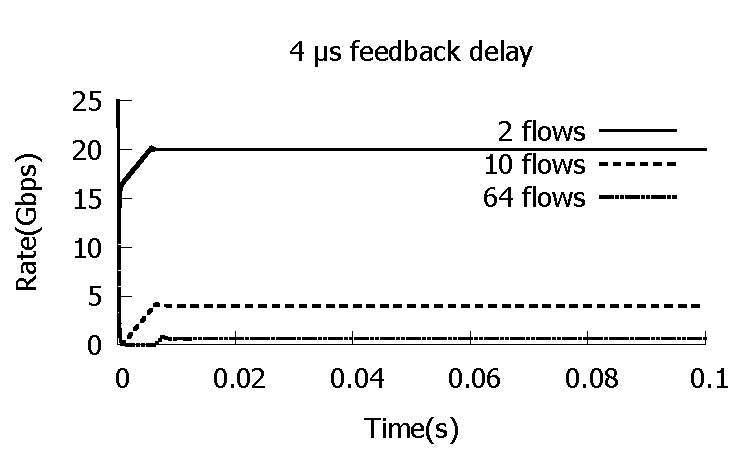
\includegraphics[width=0.49\columnwidth]{figures/stable_rate_4.pdf}}
\subfigure[] {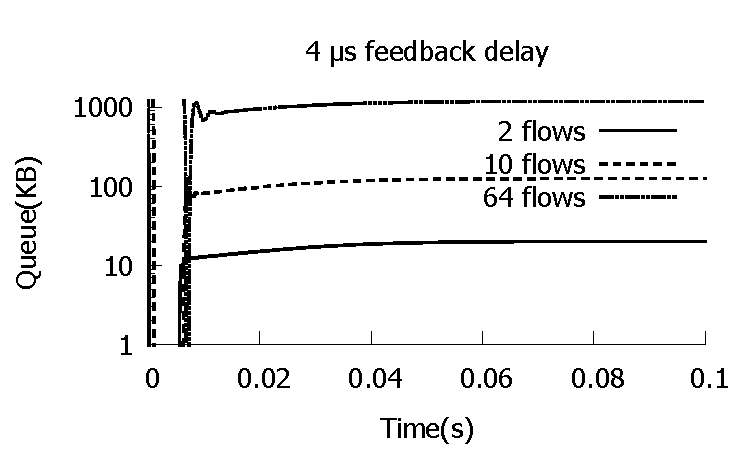
\includegraphics[width=0.49\columnwidth]{figures/stable_q_4.pdf}}
\subfigure[] {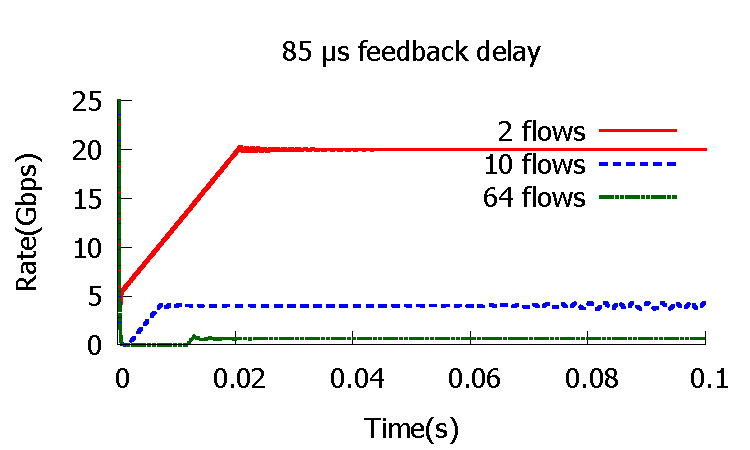
\includegraphics[width=0.49\columnwidth]{figures/stable_rate_85.pdf}}
\subfigure[] {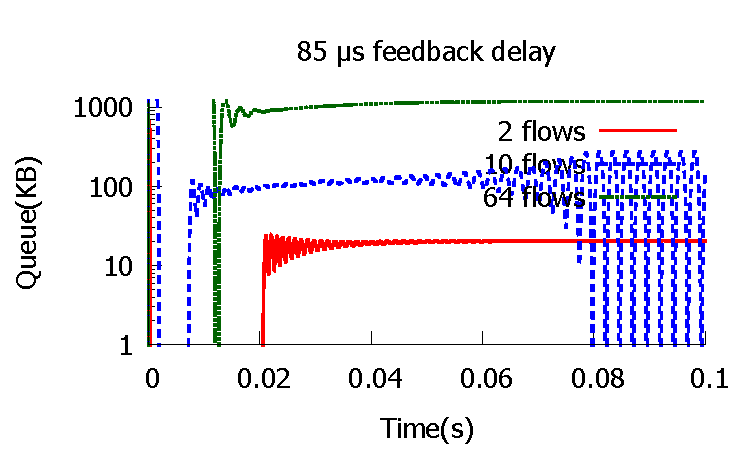
\includegraphics[width=0.49\columnwidth]{figures/stable_q_85.pdf}}
\caption{Impact of delay and number of flows on DCQCN stability}
\label{fig:dcqcn_unstable}
\end{figure}
The network operators may tune parameters to make DCQCN more stable. The two
most direct parameters are $R_{AI}$ and $K_{max}$.  Smaller $R_{AI}$ means flows
increase their rate more gentle, and stabilizes the system. Similarly, larger
$K_{max} - K_{min}$ makes rate decreasing more fine grained, because the
perturbation of queue length leads to smaller marking probability perturbation.
We show these trends in Figure~\ref{fig:dcqcn_stability}(b) and (c). With small
$R_{AI}$ and large $K_{max}$, DCQCN can be always stable even when the control
signal delay reaches 100$\mu s$, which equals to the propagation delay of a
$30KM$ cable, or $500KB$ queuing delay. Such large delay is rarely seen in
today's datacenter networks.

Here we want to point out that tuning $R_{AI}$ and $K_{max}$ is a trade-off
between stability and latency. Smaller $R_{AI}$ makes flows ramp up their rates
slower, and larger $K_{max}$ leads to larger queue length. In most cases, the
default parameters strike a good enough balance between stability and latency.

\subsection{Convergence}

\begin{figure}[t]
\center
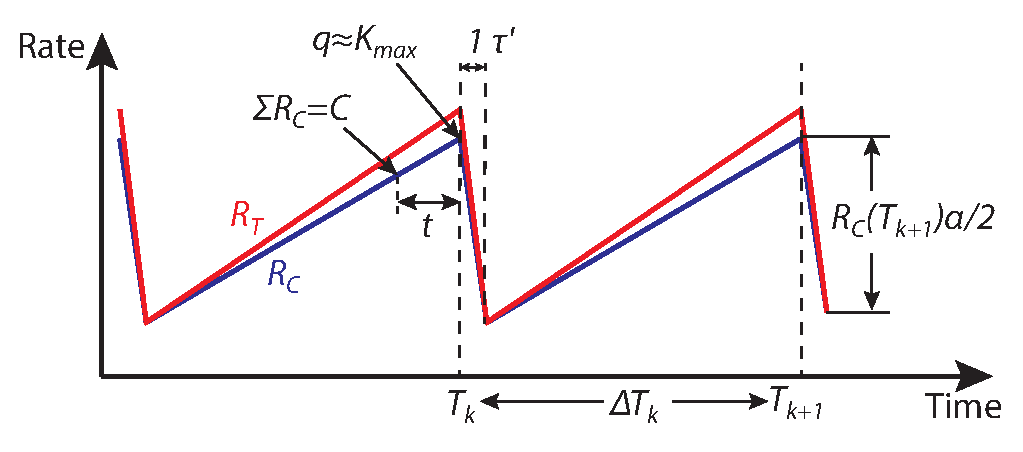
\includegraphics[width=0.4\textwidth]{figures/dcqcn_convergence.eps}
\caption{DCQCN flow rate update.}
\label{fig:dcqcn_convergence}
\end{figure}

In Section~\ref{sec:dcqcn_stability}, we show that, in reasonable paraemter ranges, 
DCQCN is stable {\em after} flows converge to the unique fixed point. However,
questions remain unanswered: do flows always converge to the fair share, and how fast
do flows converge? 

We answer this by analyzing a discrete model of the rate adjustment at the sender. In
DCQCN default parameters, the Timer $T$ and $\alpha$ update interval $\tau '$ are both 
equal to $55\mu s$. Thus, we use $\tau '$ as the unit of time. The process of DCQCN
rate updating is similar to TCP AIMD, as shown in Figure~\ref{fig:dcqcn_convergence}.
The flows get the peak rates at $T_k$. For simplicity, we assume all flows get to the peak
at the same time, which is likely to happen because the queue peak at the bottleneck 
leads to high marking probability for all flows. When the flow gets ECN marks at $T_k$,
it reduces its rate in one unit of time, then starts multiple consecutive additive rate 
increases on $R_T^{(i)}$:\footnote{For simplicity, we omit hyper-increase and fast-recover phases, 
which shall help flows converge even faster.}

\begin{equation}
\small
R_T^{(i)}({T_{k + 1}}) = \left( {1 - \frac{{{\alpha ^{(i)}}({T_k})}}{2}} \right)R_C^{(i)}({T_k}) + \left( {\Delta {T_k} - 1} \right){R_{AI}}
\label{eq:converge_rc}
\end{equation}

where $\Delta {T_k} \buildrel \Delta \over = {T_{k + 1}} - {T_k}$. During the consecutive 
additive rate increase, $R_C^{(i)}$ and $R_T^{(i)}$ have following relationship according 
to DCQCN's definition:

\begin{equation}
\small
\begin{array}{l}
R_C^{(i)}(t + 1) = \frac{1}{2}\left( {R_C^{(i)}(t) + R_T^{(i)}(t + 1)} \right)\\
R_T^{(i)}(t + 1) = R_T^{(i)}(t) + {R_{AI}}
\end{array}
\end{equation}

Subtract one of the above by the other one, we get:

\begin{equation}
\small
\begin{array}{l}
R_C^{(i)}(t + n) - R_T^{(i)}(t + n) + {R_{AI}}\\
 = \frac{1}{2}\left( {R_C^{(i)}(t + n - 1) - R_T^{(i)}(t + n - 1) + {R_{AI}}} \right)\\
 = ... = {\left( {\frac{1}{2}} \right)^n}\left( {R_C^{(i)}(t) - R_T^{(i)}(t) + {R_{AI}}} \right)
\end{array}
\end{equation}

From this, we know that with a consecutive additive rate increase phase, $R_T^{(i)} - R_C^{(i)}$
will converge towards $R_{AI}$ exponentially. In common cases, the step of additive increase
$\Delta {T_k} - 1$ is easily larger than 10, sometimes even 100, as we shall see soon. Therefore,
we can safely estimate $R_T^{(i)}$ by:

\begin{equation}
\small
R_T^{(i)}({T_k}) \approx R_C^{(i)}({T_k}) + {R_{AI}},\forall k = 1,2,...
\end{equation}

Back to Equation~\ref{eq:converge_rc}, we must know $\alpha ^{(i)}({T_k})$ and $\Delta T_k$ to 
further analyze the flow rates. During $\Delta T_k$, $\alpha ^{(i)}({T_k})$ has one increase
and $\Delta T_k - 1$ decrease, as defined by DCQCN:

\begin{equation}
\small
{\alpha ^{(i)}}({T_{k + 1}}) = {(1 - g)^{\Delta {T_k} - 1}}\left( {(1 - g){\alpha ^{(i)}}({T_k}) + g} \right)
\label{eq:converge_alpha}
\end{equation}

For another flow, {\em e.g.,} the $j$th flow, we can simply rewrite above equation by replacing 
$(i)$ with $(j)$. We subtract the equation of $j$th flow from the equation of $i$th flow, we get:

\begin{equation}
\small
\begin{array}{l}
{\alpha ^{(i)}}({T_{k + 1}}) - {\alpha ^{(j)}}({T_{k + 1}}) = {(1 - g)^{\Delta {T_k}}}\left( {{\alpha ^{(i)}}({T_k}) - {\alpha ^{(j)}}({T_k})} \right)\\
 = ... = {(1 - g)^{\sum\nolimits_{l = 0}^k {\Delta {T_l}} }}\left( {{\alpha ^{(i)}}({T_0}) - {\alpha ^{(j)}}({T_0})} \right)
\end{array}
\end{equation}

This tells us the difference of $\alpha^{(i)}$ of different flows will quickly decrease exponentially. So $\alpha^{(i)}$
of different flows will converge to the same value, and the converging speed is determined by $g$ and
$\Delta T_k$. 

Once the $\alpha$ of different flows converge to the same value $\alpha(T_{k'})$ at $T_{k'}$, we can show 
the rates $R_C$ converge afterwards. We rewrite the any $j$th flow's Equation~\ref{eq:converge_rc}, and subtract it 
from Equation~\ref{eq:converge_rc}, we get:

\begin{equation}
\small
\begin{array}{l}
R_C^{(i)}({T_{k + 1}}) - R_C^{(j)}({T_{k + 1}}) = \left( {1 - \frac{{\alpha ({T_k})}}{2}} \right)\left( {R_C^{(i)}({T_k}) - R_C^{(j)}({T_k})} \right)\\
 = ... = \prod\limits_{l = k'}^k {\left( {1 - \frac{{\alpha ({T_l})}}{2}} \right)} \left( {R_C^{(i)}({T_{k'}}) - R_C^{(j)}({T_{k'}})} \right)
\end{array}
\label{eq:converge}
\end{equation}

As long as $\alpha ({T_k})$ has a lower bound that is greater than 0, the rates $R_C$ of different flows 
converge exponentially. Before we prove this, we need to have an estimation of $\Delta T_k$ by $\alpha$.
In the period of $\Delta T_k$, after the first time unit of rate decreasing, the aggregated flow rates
will climb back to $R_C(T_{k+1})$ by $NR_{AI}$ every time unit. Thus we have:

\begin{equation}
\small\Delta {T_k} = 1 + \frac{{\sum\limits_{i = 1}^N {\left( {R_T^{(i)}({T_{k + 1}}) - \left( {1 - {\alpha ^{(i)}}({T_k})/2} \right)R_C^{(i)}({T_k})} \right)} }}{{N{R_{AI}}}}
\end{equation}

Suppose $\alpha^{(i)}$ already converged, we can largely simplify it:

\begin{equation}
\small
\begin{array}{l}
\Delta {T_k} = 1 + \frac{{\sum\limits_{i = 1}^N {R_T^{(i)}({T_{k + 1}})}  - \left( {1 - \alpha ({T_k})/2} \right)\sum\limits_{i = 1}^N {R_C^{(i)}({T_k})} }}{{N{R_{AI}}}}\\
 \approx 1 + \frac{{\left( {C + tN{R_{AI}} + N{R_{AI}}} \right) - \left( {1 - \alpha ({T_k})/2} \right)\left( {C + tN{R_{AI}}} \right)}}{{N{R_{AI}}}}\\
 = 2 + \left( {\frac{t}{2} + \frac{C}{{2N{R_{AI}}}}} \right)\alpha ({T_k})
\end{array}
\label{eq:converge_tk}
\end{equation}

Where $t$ is the time it takes the flows build up queue and get packets ECN-marked after
the aggregated flow rates exceed link capacity $C$, as shown in Figure~\ref{fig:dcqcn_convergence}.
We can estimate $t$ by the queue being built up:

\begin{equation}
\small
\begin{array}{l}
N\tau '\left( {{R_{AI}} + 2{R_{AI}} + ... + t{R_{AI}}} \right) = {Q_{ECN}} \le {K_{\max }}\\
 \Rightarrow t \le \left( { - 1 + \sqrt {1 + \frac{{8{K_{\max }}}}{{N{R_{AI}}\tau '}}} } \right)/2
\end{array}
\end{equation}

Combining Equation~\ref{eq:converge_alpha} and~\ref{eq:converge_tk}, we denote the fixed point of 
the $\alpha$ array as $\alpha^{*}$ (and corresponding $\Delta T^{*}$ from Equation~\ref{eq:converge_tk}):

\begin{equation}
\small
{\alpha ^*} = {(1 - g)^{\Delta {T^*}}}\left( {(1 - g){\alpha ^*} + g} \right)
\end{equation}

Next, we will prove:

\begin{equation}
\small
\alpha ({T_0}) > ... > \alpha ({T_k}) > \alpha ({T_{k + 1}}) > ... > {\alpha ^*} > 0
\end{equation}

Once this is proved, $\alpha ({T_k})$ has a non-zero lower bound, $R_C$ will converge exponentially.
We prove this by mathematical induction. First of all, the initial value of $\alpha$ is 1, as defined
by DCQCN. So, $\alpha ({T_0}) > {\alpha ^*} > 0$. Now assuming $\alpha ({T_k}) > {\alpha ^*} > 0$, we 
prove $\alpha ({T_k}) > \alpha ({T_{k+1}}) > {\alpha ^*}$. We define $f(\alpha)$ as the RHS of 
Equation~\ref{eq:converge_alpha}:

\begin{equation}
\small
f(\alpha ) = {(1 - g)^{2 + \left( {\frac{t}{2} + \frac{C}{{2N{R_{AI}}}}} \right)\alpha }}\left( {(1 - g)\alpha  + g} \right)
\end{equation}

By analyzing the derivative of $f(\alpha )$, it is not hard to see that with common parameter 
settings, $f(\alpha )$ is monotonically increasing. Therefore, 

\begin{equation}
\small
\alpha ({T_{k + 1}}) = f\left( {\alpha ({T_k})} \right) > f\left( {{\alpha ^*}} \right) = {\alpha ^*}
\end{equation}

In addition, because $\alpha ({T_k}) > {\alpha ^*}$, $\Delta {T_k} > \Delta {T^*}$. 
Then $\alpha^{*}$ satisfies:

\begin{equation}
\small
{\alpha ^*} > {(1 - g)^{\Delta {T_k}}}\left( {(1 - g){\alpha ^*} + g} \right)
\end{equation}

Subtract it from Equation~\ref{eq:converge_alpha}, we see $\alpha ({T_k})$ is exponentially 
converging to $\alpha ^*$:

\begin{equation}
\small
0 < \alpha ({T_{k + 1}}) - {\alpha ^*} < {(1 - g)^{\Delta {T_n}}}\left( {\alpha ({T_k}) - {\alpha ^*}} \right)
\end{equation}

This concludes our proof. Combining Equation~\ref{eq:converge_rc}, we know that $R_C$ is 
converging at the rate of at least $( {1 - \frac{{{\alpha ^{*}}}}{2}} )^k$.

\begin{figure}[t]
\center
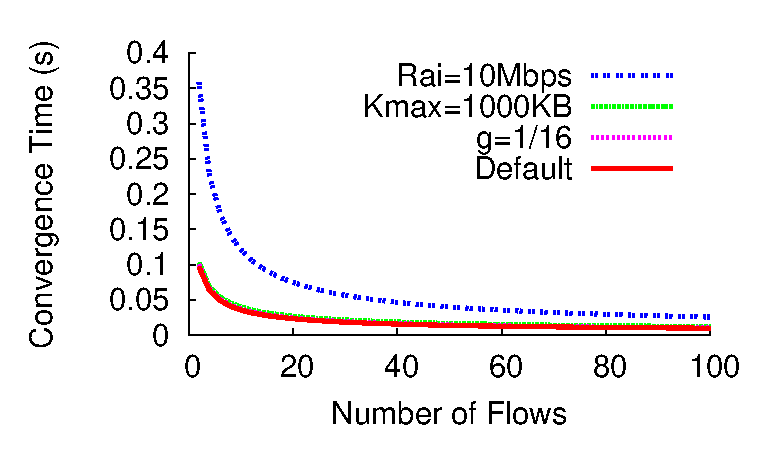
\includegraphics[width=0.4\textwidth]{figures/dcqcn_convergence_time.eps}
\caption{DCQCN flow convergence time.}
\label{fig:dcqcn_convergence_time}
\end{figure}

\para{Convergence speed.} Here we derive the upper bound of flow convergence time in DCQCN.
In the above analysis, the convergence has two phases: 1) $\alpha ^{(i)}$ converge to the 
same value (not necessarily at $\alpha^*$); 2) $R_C^{(i)}$ converge along with $\alpha -> \alpha^*$. 
In practice, the flows that encounter congestion for the first time all have the same initial
value of 1. Therefore, we mainly focus on the second phase. We define "converged" as the rate
difference of any two flows is no more than 10\% of expected fair share.

For the upper bound, we consider several worst-case assumptions. First, we assume flows start
at extremely different rates, {\em i.e.,}, some flows at 0 and some flows at 40Gbps. Second, the value of 
$\alpha ({T_k})$ is $\alpha ^*$. As shown above, $\alpha ({T_k}) > \alpha ^*$, the flows 
converge faster than our estimation in practice, given the term $(1 - \alpha /2)^T$ in Equation~\ref{eq:converge}.
Finally, the switch does not mark ECN until the queue length hits $K_{max}$, opposed to
using RED. The convergence time can be estimated by solving the following inequality of $x$: 

\begin{equation}
\small
{\left( {1 - \frac{{{\alpha ^*}}}{2}} \right)^{\frac{x}{{{T^*}\tau '}}}}C \le 10\% \frac{C}{N}
\end{equation}

We solve this using numeric approaches for different parameter settings, and show the results
in Figure~\ref{fig:dcqcn_converge_time}. We see that DCQCN converge within 100ms, and the convergence
time decreases quickly as the number of flow increases. We also test different parameters, 
including $R_{AI}$, $K_{max}$ and $g$. We found that convergence time is mostly determined by
$R_{AI}$, and much less affected by the other two. 
